\documentclass{article}

%%%%%%%%%%%%%%%%%%%%%%%%%
% Packages & Macros
%%%%%%%%%%%%%%%%%%%%%%%%%

% For including graphics
\usepackage{graphicx}

% For title page
\usepackage{datetime}
\newdateformat{monthyeardate}{\monthname[\THEMONTH] \THEYEAR}

% For supporting linking
\usepackage{hyperref}
\hypersetup{colorlinks,urlcolor=blue,linkcolor=blue}

% For supporting subfigure captions
\usepackage{subcaption}

% For making text listings (Figure 7 and 8)
\usepackage{listings}

% For string comparison in macros
\usepackage{etoolbox} 

% For table colouring (in command line tables)
%\usepackage{colortbl}

%%%%%%%%%%%%%%%%%%%%%%%%%
% Tool-Specific Macros
%%%%%%%%%%%%%%%%%%%%%%%%%
\usepackage{xspace}

\newcommand{\args}[1] {\textit{#1}}
\newcommand{\cmd}[1] {\texttt{#1}}     % Use for command window commands, e.g., \cmd{svn up}
\newcommand{\block}[1] {\textsf{#1}}   % Use for Simulink block names, e.g., \cmd{Subsystem1}
\newcommand{\signal}[1] {\textsf{#1}}   % Use for Simulink block names, e.g., \cmd{Subsystem1}
\newcommand{\ring}[1] {\textsf{#1}} 	 % Use for files names and paths
\newcommand{\keyword}[1] {\texttt{#1}} % Use for keywords of programming languages, e.g., \keyword{while}
\newcommand{\file}[1] {\texttt{#1}} 	 % Use for files names and paths
\newcommand{\param}[1] {\textsf{#1}}   % Use for block parameter names, e.g., \param{BlockType}

% Matlab Products
\newcommand{\matlab}{\textsc{Matlab}\@\xspace}
\newcommand{\Matlab}{\textsc{Matlab}\@\xspace}
\newcommand{\Simulink}{Simulink\@\xspace}
\newcommand{\simulink}{Simulink\@\xspace}
\newcommand{\SDV}{Simulink Design Verifier\@\xspace}
\newcommand{\mpath}{\Matlab search path\@\xspace}

% Block Names (not BlockType)
\newcommand{\ds}{\block{Data Store}\@\xspace}
\newcommand{\DSM}{\block{Data Store Memory}\@\xspace}
\newcommand{\DSR}{\block{Data Store Read}\@\xspace}
\newcommand{\DSW}{\block{Data Store Write}\@\xspace}
\newcommand{\DSRW}{\block{Data Store Read/Write}\@\xspace}
\newcommand{\DSMRW}{\block{Data Store Memory/Read/Write}\@\xspace}

\newcommand{\goto}{\block{Goto}\@\xspace}
\newcommand{\from}{\block{From}\@\xspace}

\newcommand{\inport}{\block{Inport}\@\xspace}
\newcommand{\outport}{\block{Outport}\@\xspace}

\newcommand{\argin}{\block{ArgIn}\@\xspace}
\newcommand{\argout}{\block{ArgOut}\@\xspace}

\newcommand{\constant}{\block{Constant}\@\xspace}
\newcommand{\ground}{\block{Ground}\@\xspace}
\newcommand{\subsystem}{\block{Subsystem}\@\xspace}

\newcommand{\logic}{\block{Logical Operator}\@\xspace}
\newcommand{\relational}{\block{Relational Operator}\@\xspace}
\newcommand{\ifblk}{\block{If}\@\xspace}
\newcommand{\switch}{\block{Switch}\@\xspace}
\newcommand{\merge}{\block{Merge}\@\xspace}

\newcommand{\docblock}{\block{DocBlock}\@\xspace}

\newcommand{\trigger}{\block{Trigger}\@\xspace}

\newcommand{\simfunc}{\block{Simulink Function}\@\xspace}
\newcommand{\simfunccaller}{\block{Function Caller}\@\xspace}

\newcommand{\toworkspace}{\block{To Workspace}\@\xspace}
\newcommand{\fromworkspace}{\block{From Workspace}\@\xspace}

\newcommand{\tofile}{\block{To File}\@\xspace}
\newcommand{\fromfile}{\block{From File}\@\xspace}

\newcommand{\fromspreadsheet}{\block{From Spreadsheet}\@\xspace}

\newcommand{\modelref}{\block{Model Reference}\@\xspace}
\newcommand{\library}{\block{Library}\@\xspace}
\newcommand{\librarylink}{\block{Library Link}\@\xspace}

% Commonly used parameters
\newcommand{\AND}{\param{AND}\@\xspace}
\newcommand{\OR}{\param{OR}\@\xspace}
\newcommand{\NOT}{\param{NOT}\@\xspace}
\newcommand{\NOR}{\param{NOR}\@\xspace}
\newcommand{\NAND}{\param{NAND}\@\xspace}
\newcommand{\XOR}{\param{XOR}\@\xspace}
\newcommand{\NXOR}{\param{NXOR}\@\xspace}

% Common Abbreviations
% Example
\newcommand{\eg}{\textrm{e.g.,}\@\xspace}

% That Is To Say
\newcommand{\ie}{\textrm{i.e.,}\@\xspace}

% And So On
\newcommand{\etc}{\textrm{etc.}\@\xspace}

% And Others
\newcommand{\etal}{\textrm{et al.}\@\xspace}

% With Respect To
\newcommand{\wrt}{\textrm{w.r.t.}\@\xspace}

% Vice Versa
\newcommand{\vrsa}{\textrm{vice versa}\@\xspace}

% Symbols

\usepackage{amssymb}
\newcommand{\checkbox}{\makebox[0pt][l]{$\square$}\raisebox{.15ex}{\hspace{0.1em}$\checkmark$}}%
\newcommand{\uncheckbox}{$\square$~}%


\newcommand{\ToolName}{Simulink Module Tool\@\xspace}

\newcommand{\menu}[1]{%
	\ifstrequal{#1}{1}{Call Function}{}%
  \ifstrequal{#1}{2}{Create Function Caller}{}%
	\ifstrequal{#1}{3}{Change Function Scope}{}%
	\ifstrequal{#1}{4}{Check Guidelines}{}%
	\ifstrequal{#1}{5}{Show Interface}{}%
	\ifstrequal{#1}{6}{Print Interface}{}%
	\ifstrequal{#1}{7}{Print Dependencies}{}%
	\ifstrequal{#1}{8}{Delete Interface}{}%
}

\newcommand{\func}[1]{%
	\ifthenelse{\equal{#1}{1}}{CreateFcnCallerLocal}{}%
	\ifthenelse{\equal{#1}{2}}{CreateFcnCaller}{}%
	\ifthenelse{\equal{#1}{3}}{setFcnScope}{}%
	\ifthenelse{\equal{#1}{4}}{?}{}%
	\ifthenelse{\equal{#1}{5}}{?}{}%
	\ifthenelse{\equal{#1}{6}}{?}{}%
}

\newcommand{\demoName}{\cmd{Demo}\@\xspace}

%%%%%%%%%%%%%%%%%%%%%%%%%
% Document
%%%%%%%%%%%%%%%%%%%%%%%%%

\begin{document}

%%%%%%%%%%%%%%%%%%%%%%%%%%%%%%%%%%%%%%%%%%%%%%%%%%%%%%%%%%%%%%%%%%%
% Title Page
%%%%%%%%%%%%%%%%%%%%%%%%%%%%%%%%%%%%%%%%%%%%%%%%%%%%%%%%%%%%%%%%%%%
\title{\ToolName}
\date{\monthyeardate\today}
\maketitle
\vfill

%\begin{figure}
%	\centering
%	
\includegraphics[]{../../common/McSCert_Logo.pdf} \\
%	McMaster Centre for Software Certification (McSCert)
%\end{figure}

\newpage

%%%%%%%%%%%%%%%%%%%%%%%%%%%%%%%%%%%%%%%%%%%%%%%%%%%%%%%%%%%%%%%%%%%
% Table of Contents
%%%%%%%%%%%%%%%%%%%%%%%%%%%%%%%%%%%%%%%%%%%%%%%%%%%%%%%%%%%%%%%%%%%

\tableofcontents
\newpage

%%%%%%%%%%%%%%%%%%%%%%%%%%%%%%%%%%%%%%%%%%%%%%%%%%%%%%%%%%%%%%%%%%%
% Introduction
%%%%%%%%%%%%%%%%%%%%%%%%%%%%%%%%%%%%%%%%%%%%%%%%%%%%%%%%%%%%%%%%%%%
\section{Introduction}

% Briefly, what is the tool?
% Provide any background or references.
The \ToolName performs several functions in order to support modular development for \Simulink models. A \Simulink module structure can be summarized by Figure~\ref{FIG:module}. This tool helps in scoping \simfunc{s}, displaying interfaces, and checking associated guidelines. The following sections explain each of the tool functions.

\begin{figure}
	\centering
	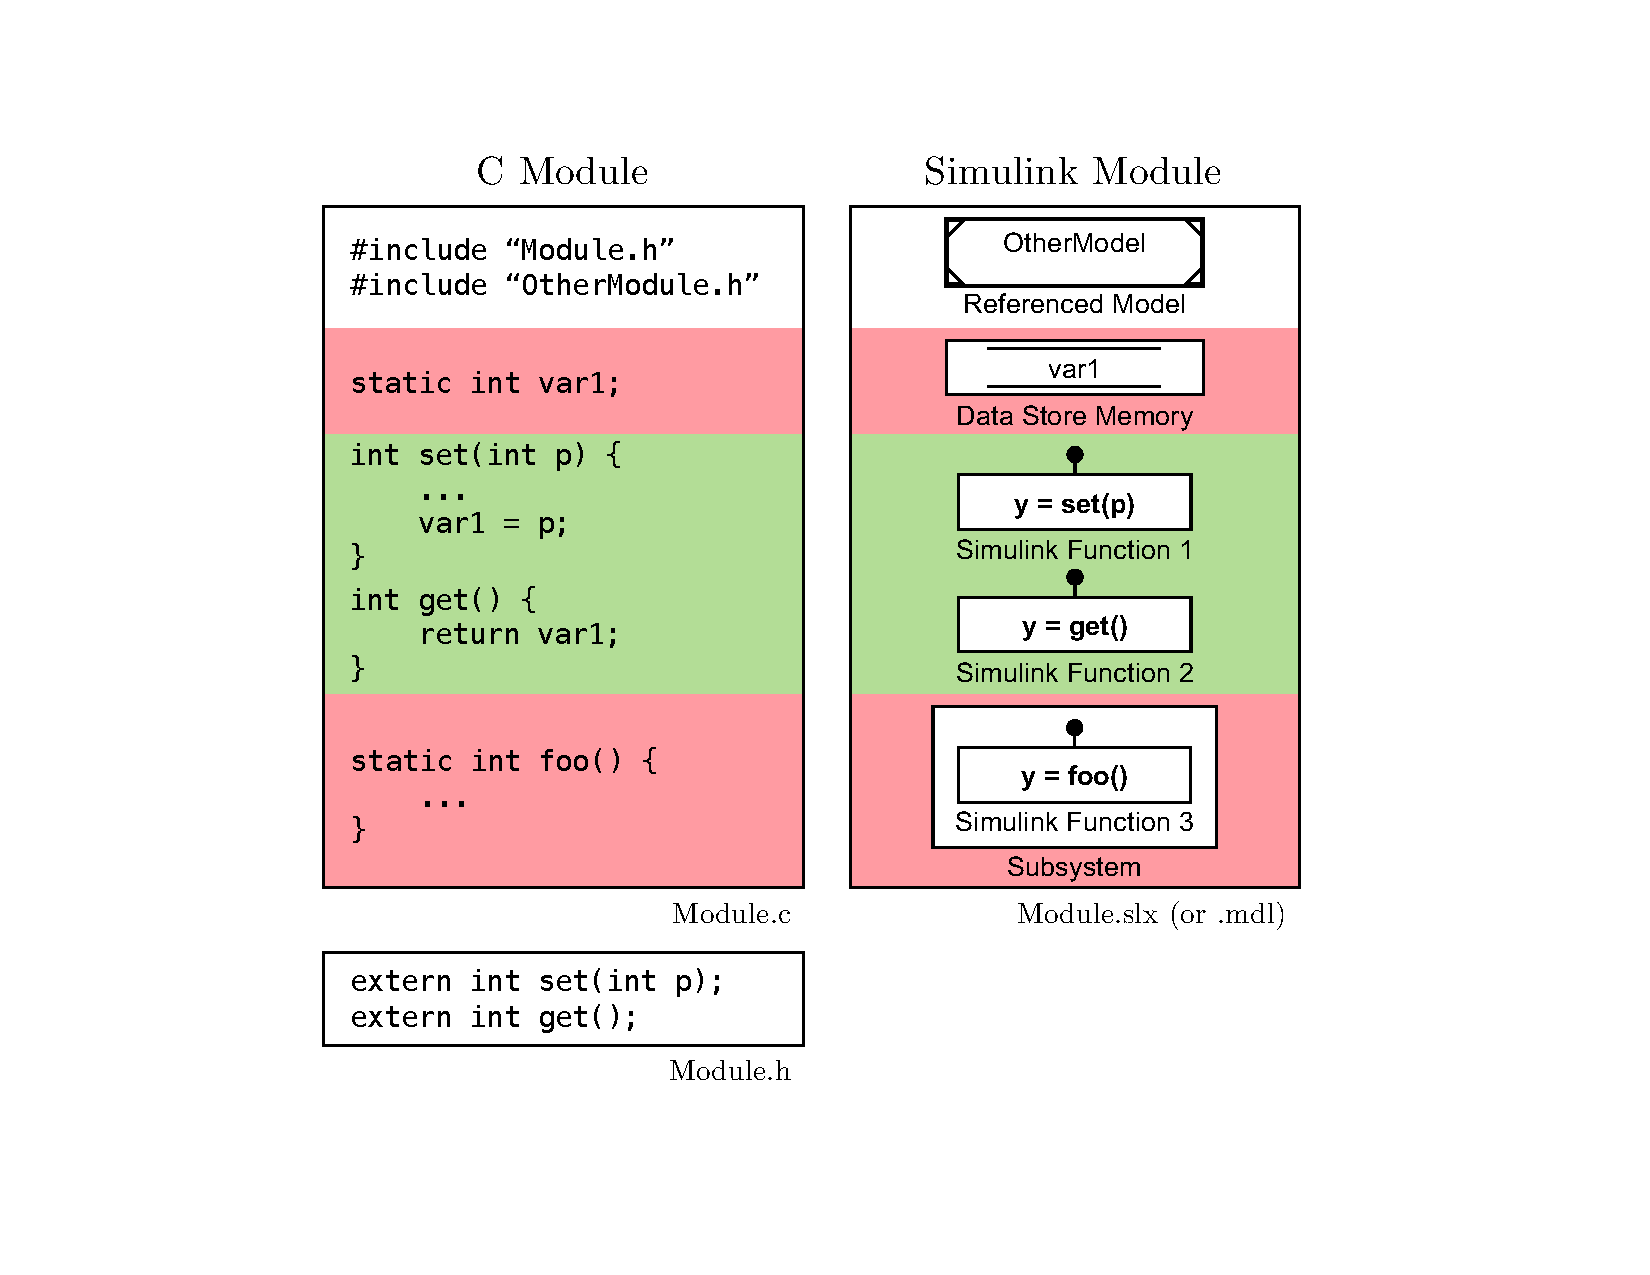
\includegraphics[width=0.75\textwidth]{../figs/Module}
	\caption{\Simulink module structure based on C.}
	\label{FIG:module}
\end{figure}

\subsection{Simulink Functions}
In \Simulink, a function can be defined via the \simfunc block, and invoked graphically via \simfunccaller blocks. In the modular programming approach to software development, a system is decomposed into modules. Each module must be able to hide information in its implementation, and only expose on the interface information what is to be shared with other modules. One can use \simfunc blocks to selectively hide or expose elements on the interface. However, a thorough understanding of the \simfunc block is necessary in order to know how the \emph{Function Visibility} parameter and location in the model impacts its accessibility and name qualification. 

The \ToolName assists developers with using \simfunc blocks in implementing \Simulink modules. The tool can automatically convert between the different scopes of \simfunc{s}, thereby changing whether it is exposed on the interface or local to the model. The tool also assists users in quickly calling \simfunc{s}, with their appropriate qualifiers, from any location in a model or parent hierarchy, as well as creating \simfunccaller blocks with their \emph{Function prototype}, \emph{Input argument specifications}, and \emph{Output argument specifications} parameters automatically populated (if possible).

\subsection{Interfaces}
A \Simulink model's interface is commonly considered to be comprised of the \inport{s} and \outport{s} of the top-level system. A module interface should make clear \emph{all} the communication of a module. The \fromfile, \fromspreadsheet, \fromworkspace blocks, and global \ds{s} that are read are also inputs to the model. Elements that are outputs of the model can also include \toworkspace, \tofile, and global \ds{s} that are written to. Additionally, \simfunc definitions can be exported from a model. %A complete definition of a \Simulink module interface is presented in~\cite{paper}.

The \ToolName automatically extracts the interface of a \Simulink module and either represents it in the the root of the \Simulink module, or prints the interface to the Command Window.

\subsection{Dependencies}

A \Simulink model can have many dependencies in the form of \modelref{s}, \library linked blocks, and data dictionaries. These reside outside of the \Simulink module, but are necessary in order to be able to simulate and code generate the model.

The \ToolName examines the model, determines which dependencies exist, and prints a list to the Command Window.

\subsection{Guidelines}
Guidelines relating to \simfunc{s} and interfaces are presented in~\cite{paper}. Tables \ref{tbl:guideline1}, \ref{tbl:guideline2}, \ref{tbl:guideline3}, and \ref{tbl:guideline4} outline the guidelines, and the tool automates the checking of these guidelines.

% Is there more information?
%\subsection*{More Information}
%For more information on the tool and how it can be used in model-based development with \Simulink, please the paper:

%\vspace{1em}
%Monika Jaskolka, Vera Pantelic, Mark Lawford, and Alan Wassyng, ``Supporting Modularity for \Simulink Models", 2019, \textit{(Manuscript in Preparation)}.

% Is there more information?
%\subsection*{More Information}
%For more about the theoretical background of ... and how they can be used, an interested reader is referred to:
%
%\vspace{1em}
% <citation goes here>

\newpage	
%%%%%%%%%%%%%%%%%%%%%%%%%%%%%%%%%%%%%%%%%%%%%%%%%%%%%%%%%%%%%%%%%%%
% How to Use the Tool
%%%%%%%%%%%%%%%%%%%%%%%%%%%%%%%%%%%%%%%%%%%%%%%%%%%%%%%%%%%%%%%%%%%
\section{How to Use the Tool}
This section describes what must be done to setup the \ToolName, as well as how to use the tool.

%---------------------------------------
% What needs to be done before the tool can be used? 
% What needs to be done to a model in order for it to work on said model?
%---------------------------------------
\subsection{Prerequisites and Installation}

\begin{enumerate}
\item For full use of the tool, please use \matlab/\Simulink R2017b or newer.\footnote{Simulink functions were introduced in R2014b. The \emph{Function Visibility} parameter was introduced in R2017b.}

\item To install the tool,
	\begin{enumerate}
		\item from a \file{.zip} file --- unzip the contents into your desired location. Ensure the unzipped folder and subfolders are present in your \mpath, or add them if they are not present. Run \href{https://www.mathworks.com/help/simulink/ug/registering-customizations.html}{sl\_refresh\_customizations} to refresh the Context Menu. 
		\item from a \file{.mltbx} file --- simply open \Matlab and double-click on the file. Your \mpath should be automatically configured.
		\item from the files only --- add the folders and subfolders to your \mpath. Run \href{https://www.mathworks.com/help/simulink/ug/registering-customizations.html}{sl\_refresh\_customizations} to refresh the Context Menu.
	\end{enumerate}
	\begin{itemize}
		\item \textit{Note:} If running the command ``\cmd{which AutoLayout}'' indicates that the script is not found, then the tool needs to be added to the \mpath.
		For information on adding files to the \mpath, please see the \href{https://www.mathworks.com/help/matlab/matlab_env/add-remove-or-reorder-folders-on-the-search-path.html}{MathWorks documentation}.
	\end{itemize}
\item Ensure your model is open and unlocked.
\end{enumerate}

%---------------------------------------
% How/when do you access the tool?
%---------------------------------------
\subsection{Getting Started}
The tool can be used via the \Simulink Context Menu, which can be viewed by right-clicking in a model. The following options can be available, depending on what is selected in the model, and which version of \Matlab/\Simulink is used.

\noindent
Options available when no blocks are selected are (Figure~\ref{FIG:none_selected}):
\begin{itemize}
	\item \emph{\menu{1}} %-- R2014b+
	\item \emph{\menu{4}}
	\item \emph{\menu{5}} %-- R2016a+
	\item \emph{\menu{6}} %-- R2016a+
	\item \emph{\menu{8}} %-- Only when an interface is shown in the module.
	\item \emph{\menu{7}} 
\end{itemize}

\noindent
Options available when one or more \simfunc blocks are selected are (Figure~\ref{FIG:simfunc_selected}):
\begin{itemize}
	\item \emph{\menu{3}} %-- R2017b+
	\item \emph{\menu{2}} %-- R2014b+
\end{itemize}

\begin{figure}[!htb]
    \centering
    \begin{subfigure}[b]{\textwidth}
    \centering
    	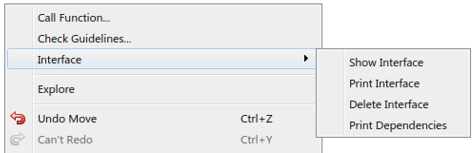
\includegraphics[width=0.65\textwidth]{../figs/ContextMenu1}
        \caption{Menu options when no functions are selected.}
        \label{FIG:none_selected}
    \end{subfigure}
    
		\vspace{1em}%
		
    \begin{subfigure}[b]{\textwidth}
    \centering
			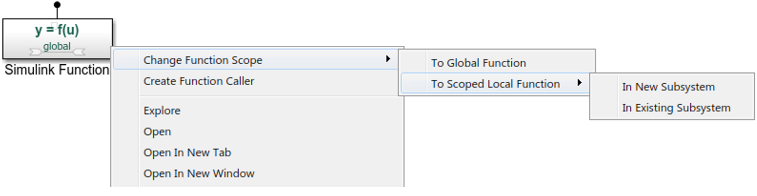
\includegraphics[width=\textwidth]{../figs/ContextMenu2}
        \caption{Menu options when one or more functions are selected.}
        \label{FIG:simfunc_selected}
    \end{subfigure}
	\caption{Simulink Context Menu with context-dependant tool options visible.}
	\label{FIG:contextMenu}
\end{figure}

%---------------------------------------
% What are the main uses of the tool?
%---------------------------------------
\newpage
\subsection{Functionality}
This section describes the tool functionality when it is used from the \Simulink Context Menu (Figure~\ref{FIG:contextMenu}). 

%We will demonstrate on the model shown in Figure~\ref{FIG:examplemodel}.

%\begin{figure}
%  \includegraphics[width=\columnwidth]{../figs/Demo}
%  \caption{A \Simulink model (in Interface Display view).}
%  \label{FIG:examplemodel}
%\end{figure}

%-------------------------
\subsubsection{\menu{1}}
%-------------------------
\emph{Note: This option is not available in versions prior to R2014b.}

Right-clicking anywhere in the model and then selecting \cmd{\menu{1}} from the Context Menu will display the user interface shown in Figure~\ref{FIG:gui}. The listbox shows all \simfunc{s} that can be called from that location in the model. Select a function, press OK, and a \simfunccaller will be created with its \keyword{Prototype}, \keyword{Input argument specifications}, and \keyword{Output argument specifications} parameters automatically populated. 

This function automates the following manual steps:
\begin{enumerate}
	\item Drag and drop a \simfunc block from the User-Defined Functions library into the model.
	\item Open the \simfunc block parameters.
	\item Enter a \keyword{Prototype} from those available.
	\item Determine the input and output types and dimensions. Enter them into the \keyword{Input argument specifications} and \keyword{Output argument specifications} fields in the appropriate formatting.
\end{enumerate}
Moreover, it allows you to see which \simfunc{s} are available (\ie in scope) from any location in the model.

\begin{figure}[htb]
	\centering
	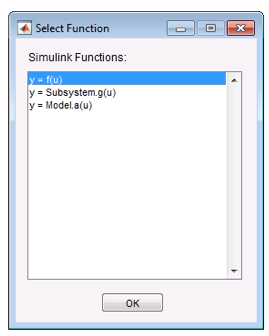
\includegraphics[width=0.5\textwidth]{../figs/GUI}
	\caption{Select Function interface.}
	\label{FIG:gui}
\end{figure}

%-------------------------
\subsubsection{\menu{3}}
%-------------------------
\emph{Note: This option is not available in versions prior to R2017b.}

Right-clicking directly on one or more \simfunc blocks and then selecting \cmd{\menu{3}} from the Context Menu, will display options for changing the scope of the functions. An example is shown in Figure~\ref{FIG:demo2}. 

The scope of a Simulink function, \ie where it can be used, is determined by both its hierarchal \emph{placement} in the model in which it is defined, and its \emph{Function Visibility} parameter. 
The rules for determining the scope of a \simfunc are not straightforward. When a \simfunc is given global function visibility, it can be placed anywhere in a model, and will be available for use anywhere in the model hierarchy (\ie in any subsystems or in the parent model hierarchy). When a \simfunc is given scoped function visibility, its placement in the model affects its accessibility. If placed at root level, it is accessible in the model hierarchy. The difference between a global \simfunc and a scoped \simfunc placed at the root is in the way it is called. In the latter, the function name must be qualified with the model reference block name. If the scoped \simfunc is placed in a subsystem $S$ (\ie not at the root), it is no longer available outside of the model. Instead, it is available in the parent subsystem of $S$ and any descendants. %If a scoped \simfunc being placed in an atomic subsystem, it is accessible only inside the subsystem and its descendants.

\begin{figure}
\centering
	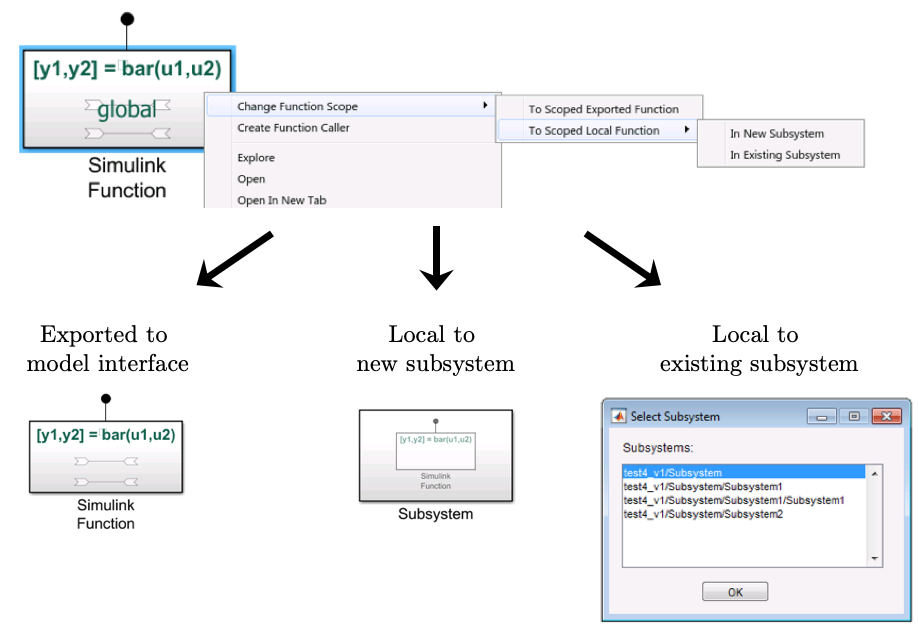
\includegraphics[width=\textwidth]{../figs/Demo2}
    \caption{Changing \simfunc scopes.}
    \label{FIG:demo2}
\end{figure}

%-------------------------
\subsubsection{\menu{2}}
%-------------------------
\emph{Note: This option is not available in versions prior to R2014b.}

Right-clicking on one or more \simfunc blocks and then selecting \cmd{\menu{2}} from the Context Menu, will automatically create corresponding \simfunccaller blocks for the selected functions. The \keyword{Prototype}, \keyword{Input argument specifications}, and \keyword{Output argument specifications} parameters of the new \simfunccaller are automatically populated. An example is shown in Figure~\ref{fig:demo1a}.

\begin{figure}[!htb]
    \centering
    \begin{subfigure}[b]{\textwidth}
    \centering
    	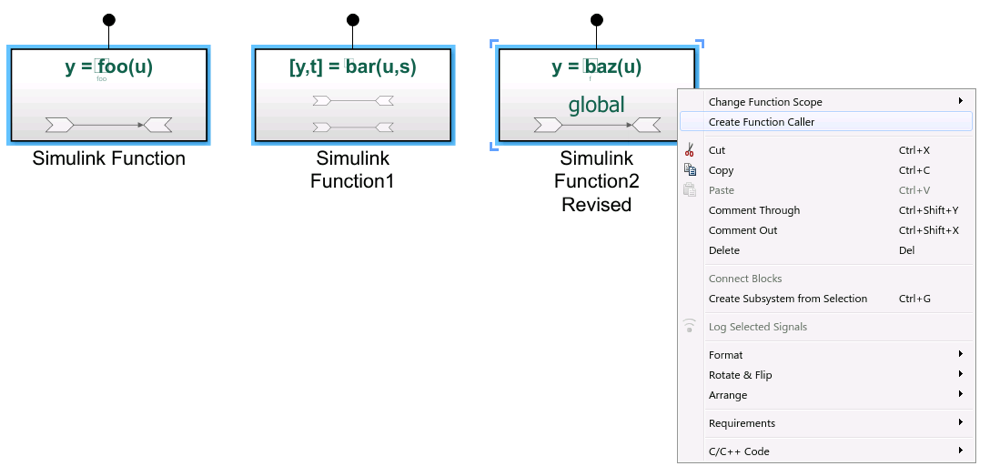
\includegraphics[width=\textwidth]{../figs/Demo1a}
        \caption{Select \menu{2} from the Context Menu.}
        \label{fig:demo1a}
    \end{subfigure}
    
		\vspace{1em}%
		
    \begin{subfigure}[b]{\textwidth}
    \centering
			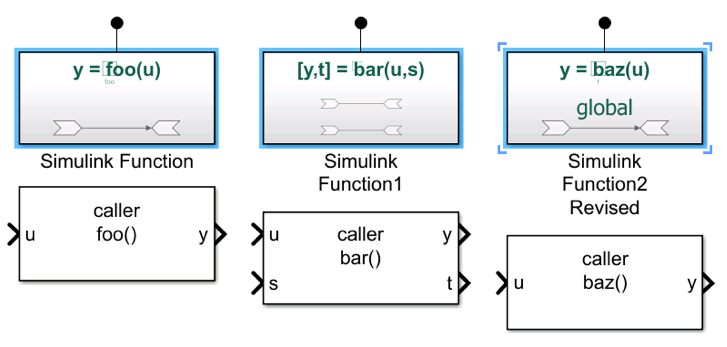
\includegraphics[width=.75\textwidth]{../figs/Demo1b}
        \caption{New function callers are added.}
        \label{fig:demo1b}
    \end{subfigure}
	\caption{Example of Simulink Function Caller creation.}
	\label{fig:demo1}
\end{figure}

\newpage
%-------------------------
\subsubsection{\menu{4}}
%-------------------------
Right-clicking anywhere in the model and then selecting \cmd{\menu{4}} from the Context Menu will display the user interface shown in Figure~\ref{FIG:guideline}. The window shows all the guidelines that can be enabled by the user, and hovering over their names with the cursor will display a brief description of the guideline. The guidelines are detailed in Tables \ref{tbl:guideline1}, \ref{tbl:guideline2}, \ref{tbl:guideline3}, and \ref{tbl:guideline4}. Select one or more guidelines to check, press OK, and the Command Window will display any violations.

\begin{figure}[htb]
	\centering
	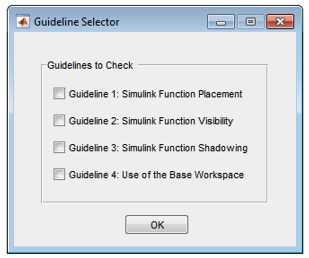
\includegraphics[width=0.5\textwidth]{../figs/GuidelineSelector}
	\caption{Select guidelines GUI.}
	\label{FIG:guideline}
\end{figure}

\begin{table}
  \centering
  \caption{Guideline on \simfunc placement.}
  \label{tbl:guideline1}
  \begin{tabular}{|l|p{30em}|}
    \hline
    ID: Title       & 1: \Simulink Function Placement \\ \hline
    Priority        & Strongly Recommended \\ \hline
    \Matlab Version & R2014b and later \\ \hline
    Description     & Position the \simfunc block in the lowest common parent of its corresponding \simfunccaller blocks. Do not position the \simfunc in the top layer for no reason. Avoid placing \simfunc blocks below their corresponding \simfunccaller blocks. \\ \hline
    Rationale			  & \checkbox Readability \newline
    							    \checkbox Verification and Validation \newline
    							  	\checkbox Workflow \newline
    								  \checkbox Code Generation \newline
    								  \uncheckbox Simulation \\ \hline
  \end{tabular}
\end{table}

\begin{table}
  \centering
  \caption{Guideline on \simfunc visibility.}
  \label{tbl:guideline2}
  \begin{tabular}{|l|p{30em}|}
    \hline
    ID: Title       & 2: \Simulink Function Visibility \\ \hline
    Priority        & Strongly Recommended \\ \hline
    \Matlab Version & R2017b and later \\ \hline
    Description     & Limit the \param{Function Visibility} parameter of the \simfunc block's trigger port to \param{scoped} if possible. \newline
    								  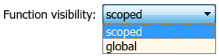
\includegraphics[scale=0.6]{../figs/FunctionVisibilityParam} \\ \hline
    Rationale			  & \checkbox Readability \newline
    							    \checkbox Verification and Validation \newline
    						 		  \checkbox Workflow \newline
    								  \checkbox Code Generation \newline
    								  \uncheckbox Simulation \\ \hline
  \end{tabular}
\end{table}

\begin{table}
  \centering
  \caption{Guideline on \simfunc shadowing.}
  \label{tbl:guideline3}
  \begin{tabular}{|l|p{30em}|}
    \hline
    ID: Title       & 3: \Simulink Function Shadowing \\ \hline
    Priority        & Strongly Recommended \\ \hline
    \Matlab Version & R2014b and later \\ \hline
    Description     & Do not place \simfunc{s} with the same name and input/output arguments within each other's scope. \\ \hline
    Rationale			  & \checkbox Readability \newline
    							    \checkbox Verification and Validation \newline
    								  \checkbox Workflow \newline
    								  \uncheckbox Code Generation \newline
    								  \uncheckbox Simulation \\ \hline
  \end{tabular}
\end{table}

\begin{table}
\centering
\caption{Guideline on using the base workspace.}
\label{tbl:guideline4}
  \begin{tabular}{|l|p{30em}|}
    \hline
    ID: Title       & 4: Use of the Base Workspace \\ \hline
    Priority        & Recommended \\ \hline
    \Matlab Version & R2006a and later \\ \hline
    Description     & Do not use the base workspace for storing, reading, or writing data that a model is dependant on. Instead, place such data in either the model workspace, if it is to be used in a single model, or a data dictionary if it is to be shared across models. This means avoiding the use of the sources,
    \begin{itemize}
    	\item \fromfile
    	\item \fromworkspace
    	\item \fromspreadsheet
    \end{itemize}
    and sinks,
    \begin{itemize}
    	\item \tofile
    	\item \toworkspace
    \end{itemize}
    as well as avoiding defining signals, types, \etc in the base workspace. \\ \hline
    Rationale			 & \checkbox Readability \newline
    							   \checkbox Verification and Validation \newline
    								 \checkbox Workflow \newline
    								 \checkbox Code Generation \newline
    								 \checkbox Simulation \\ \hline
  \end{tabular}
\end{table}

%-------------------------
\subsubsection{\menu{5} and \menu{6}}
%-------------------------
\emph{Note: This option is not available in versions prior to R2016a.}

Right-clicking anywhere in the model and then hovering over \cmd{\menu{5}} or \cmd{\menu{6}} from the Context Menu will give the user options to insert the interface representation in the model (\eg Figure~\ref{FIG:interface_visual}), or print the interface description to the Command Window (\eg Figure~\ref{FIG:interface_text}).

\begin{figure}[htb]
\begin{subfigure}[b]{.6\textwidth}
	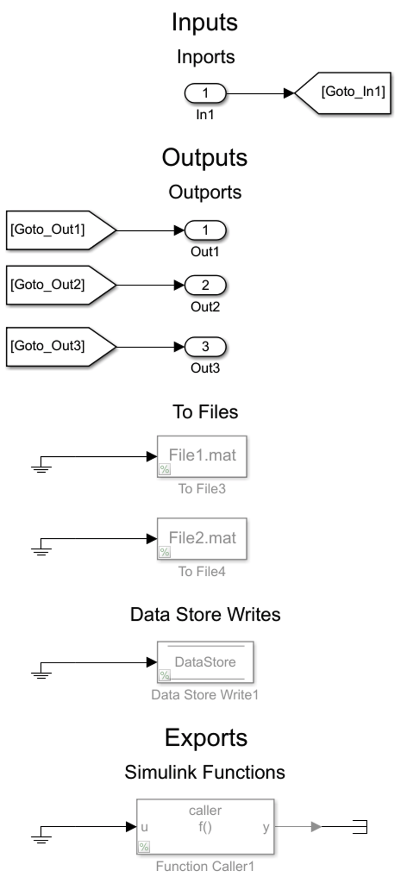
\includegraphics[height=1.4\textwidth]{../figs/Interface}
	\caption{Visual representation.}
	\label{FIG:interface_visual}
\end{subfigure}
\begin{subfigure}[b]{.4\textwidth}
\lstset{basicstyle=\footnotesize\ttfamily, keepspaces=false, columns=flexible,}
	\begin{lstlisting}
Inputs
------
Inports:
  Demo/In1, uint16, 1, 1
    
Outputs
-------
Outports:
  Demo/Out1, Inherit: auto, 1, 1
  Demo/Out2, Inherit: auto, -1, 1
  Demo/Out3, Inherit: auto, -1, Inf
To Files:
  Demo/To File1, Timeseries, N/A, 1
  Demo/To File2, Timeseries, N/A, 1
Data Store Writes:
  Demo/Data Store Write, uint16, 1, 1

Exports
-------
Simulink Functions:
  Demo/Simulink Function, 
    In:  uint16, 1, -1
    Out: uint16, 1, -1
\end{lstlisting}
\caption{Textual description.}
\label{FIG:interface_text}
\end{subfigure}
\caption{\Simulink module interface.}
\label{FIG:simulinkinterface}
\end{figure}

\paragraph{Warnings}
\begin{enumerate}
	\item This feature is only available for versions R2017b and newer. The Context Menu will have this option disabled for earlier versions. This is because the \emph{function visibility} parameter (\ie scoping) was not introduced for \simfunc{s} until R2017b.
	
		\item If a \simfunc is moved and one or more \simfunccaller{s} with the same prototype exist within its previous scope, a warning will appear in the Command Window. It is recommended that the user ensure all \simfunccaller{s} still correctly call the \simfunc. Automatic updating of \simfunccaller blocks is planned for a future version of this tool.
\end{enumerate}

%-------------------------
\subsubsection{\menu{8}}
%-------------------------
Right-clicking anywhere in the model and then selecting \cmd{\menu{8}} will delete the interface that was created using the \cmd{\menu{5}} option.

\newpage
%-------------------------
\subsubsection{\menu{7}}
%-------------------------
Right-clicking anywhere in the model and then selecting \cmd{\menu{7}} from the Context Menus will print the dependencies that the model relies on in the Command Window. Dependencies include: \modelref blocks, \library blocks, and data dictionaries. An example of the output is shown in Figure~\ref{FIG:dependencies}.

\begin{figure}[htb]
\centering
\lstset{basicstyle=\footnotesize\ttfamily, keepspaces=false, columns=flexible,}
\begin{lstlisting}
                              Model References
                              ------
                              Demo2/ControlModel
                              Demo2/Subsystem/EstimationModel
                              
                              Library Links
                              ------
                              Demo2/Subsystem2/CustomTable
                              
                              Data Dictionaries
                              ------
                              definitions.sldd
\end{lstlisting}
\caption{List of dependencies.}
\label{FIG:dependencies}
\end{figure}

%---------------------------------------
% What are the configuration options for the tool?
%---------------------------------------
%\subsection{Configuration Parameters}
%The configuration file \cmd{config.txt} is included in \cmd{\toolFolder\textbackslash src}. The following configuration parameters are utilized by the tool, and can be modified by the user in order to tailor tool functionality:
%
%\begin{itemize}
%	\item \cmd{gotofrom\_bgcolor} -- The ... 
%	\item \cmd{heading\_size} -- The ...
%\end{itemize}
%
%Please see the configuration file for more details regarding parameter usage and accepted values. These parameters can be modified with \matlab open, and do not require that \matlab be restarted for the changes to take effect.

%---------------------------------------
% What else does the tool do?
%---------------------------------------

\subsection{Errors and Warnings}
Any errors or warnings during tool use will be visible in the \matlab Command Window. %Typically, errors will be shown when the model is locked or function parameters are incorrect.


\subsection{Limitations}
A \Simulink model can depend on or interact with other files and elements via the use of Callbacks\footnote{\url{https://www.mathworks.com/help/simulink/ug/model-callbacks.html}} and S-Functions\footnote{\url{https://www.mathworks.com/help/simulink/sfg/what-is-an-s-function.html}}. Identifying these is not currently supported by the tool.

%\begin{thebibliography}{9}
%\bibitem{paper} 
%Monika Jaskolka, Vera Pantelic, Mark Lawford, and Alan Wassyng, ``Supporting Modularity for \Simulink Models", 2019, \textit{(Manuscript in Preparation)}.
%\end{thebibliography}

\end{document}